\documentclass[11pt, a4paper, twoside]{article}   	% use "amsart" instead of "article" for AMSLaTeX format

\usepackage{geometry}                		% See geometry.pdf to learn the layout options. There are lots.
\usepackage{pdfpages}
\usepackage{caption}
\usepackage{minted}
\usepackage[german]{babel}			% this end the next are needed for german umlaute
\usepackage[utf8]{inputenc}
\usepackage{color}
\usepackage{graphicx}
\usepackage{titlesec}
\usepackage{fancyhdr}
\usepackage{lastpage}
\usepackage{hyperref}
\usepackage[autostyle=false, style=english]{csquotes}
\usepackage{mathtools}
\usepackage{tabularx}
\usepackage{ulem}
% http://www.artofproblemsolving.com/wiki/index.php/LaTeX:Symbols#Operators
% =============================================
% Layout & Colors
% =============================================
\geometry{
   a4paper,
   total={210mm,297mm},
   left=20mm,
   right=20mm,
   top=20mm,
   bottom=30mm
 }	

\definecolor{myred}{rgb}{0.8,0,0}
\definecolor{mygreen}{rgb}{0,0.6,0}
\definecolor{mygray}{rgb}{0.5,0.5,0.5}
\definecolor{mymauve}{rgb}{0.58,0,0.82}

\setcounter{secnumdepth}{4}


% the default java directory structure and the main packages
\newcommand{\srcDir}{../src/AutomataForStudentsV4}
\newcommand{\imageDir}{images}
% =============================================
% Code Settings
% =============================================
\newenvironment{code}{\captionsetup{type=listing}}{}
\newmintedfile[cppSourceFile]{cpp}{
	linenos=true, 
	frame=single, 
	breaklines=true, 
	tabsize=2,
	numbersep=5pt,
	xleftmargin=10pt,
	baselinestretch=1,
	fontsize=\footnotesize
}
\newmintinline[inlineCpp]{cpp}{}
\newminted[cppSource]{cpp}{
	breaklines=true, 
	tabsize=2,
	autogobble=true,
	breakautoindent=false
}

\newcommand{\xvdash}[1]{%
  \vdash^{\mkern-10mu\scriptscriptstyle\rule[-.9ex]{0pt}{0pt}#1}%
}

% =============================================
% Page Style, Footers & Headers, Title
% =============================================
\title{Übung 3}
\author{Thomas Herzog}

\lhead{Übung 3}
\chead{}
\rhead{
\includegraphics[scale=0.10]{FHO_Logo_Students.jpg}}

\lfoot{S1610454013}
\cfoot{}
\rfoot{ \thepage / \pageref{LastPage} }
\renewcommand{\footrulewidth}{0.4pt}
% =============================================
% D O C U M E N T     C O N T E N T
% =============================================
% =============================================
% 2016.10.13: 1 
% 2016.10.14: 2
% =============================================
\pagestyle{fancy}
\begin{document}
\setlength{\headheight}{15mm}
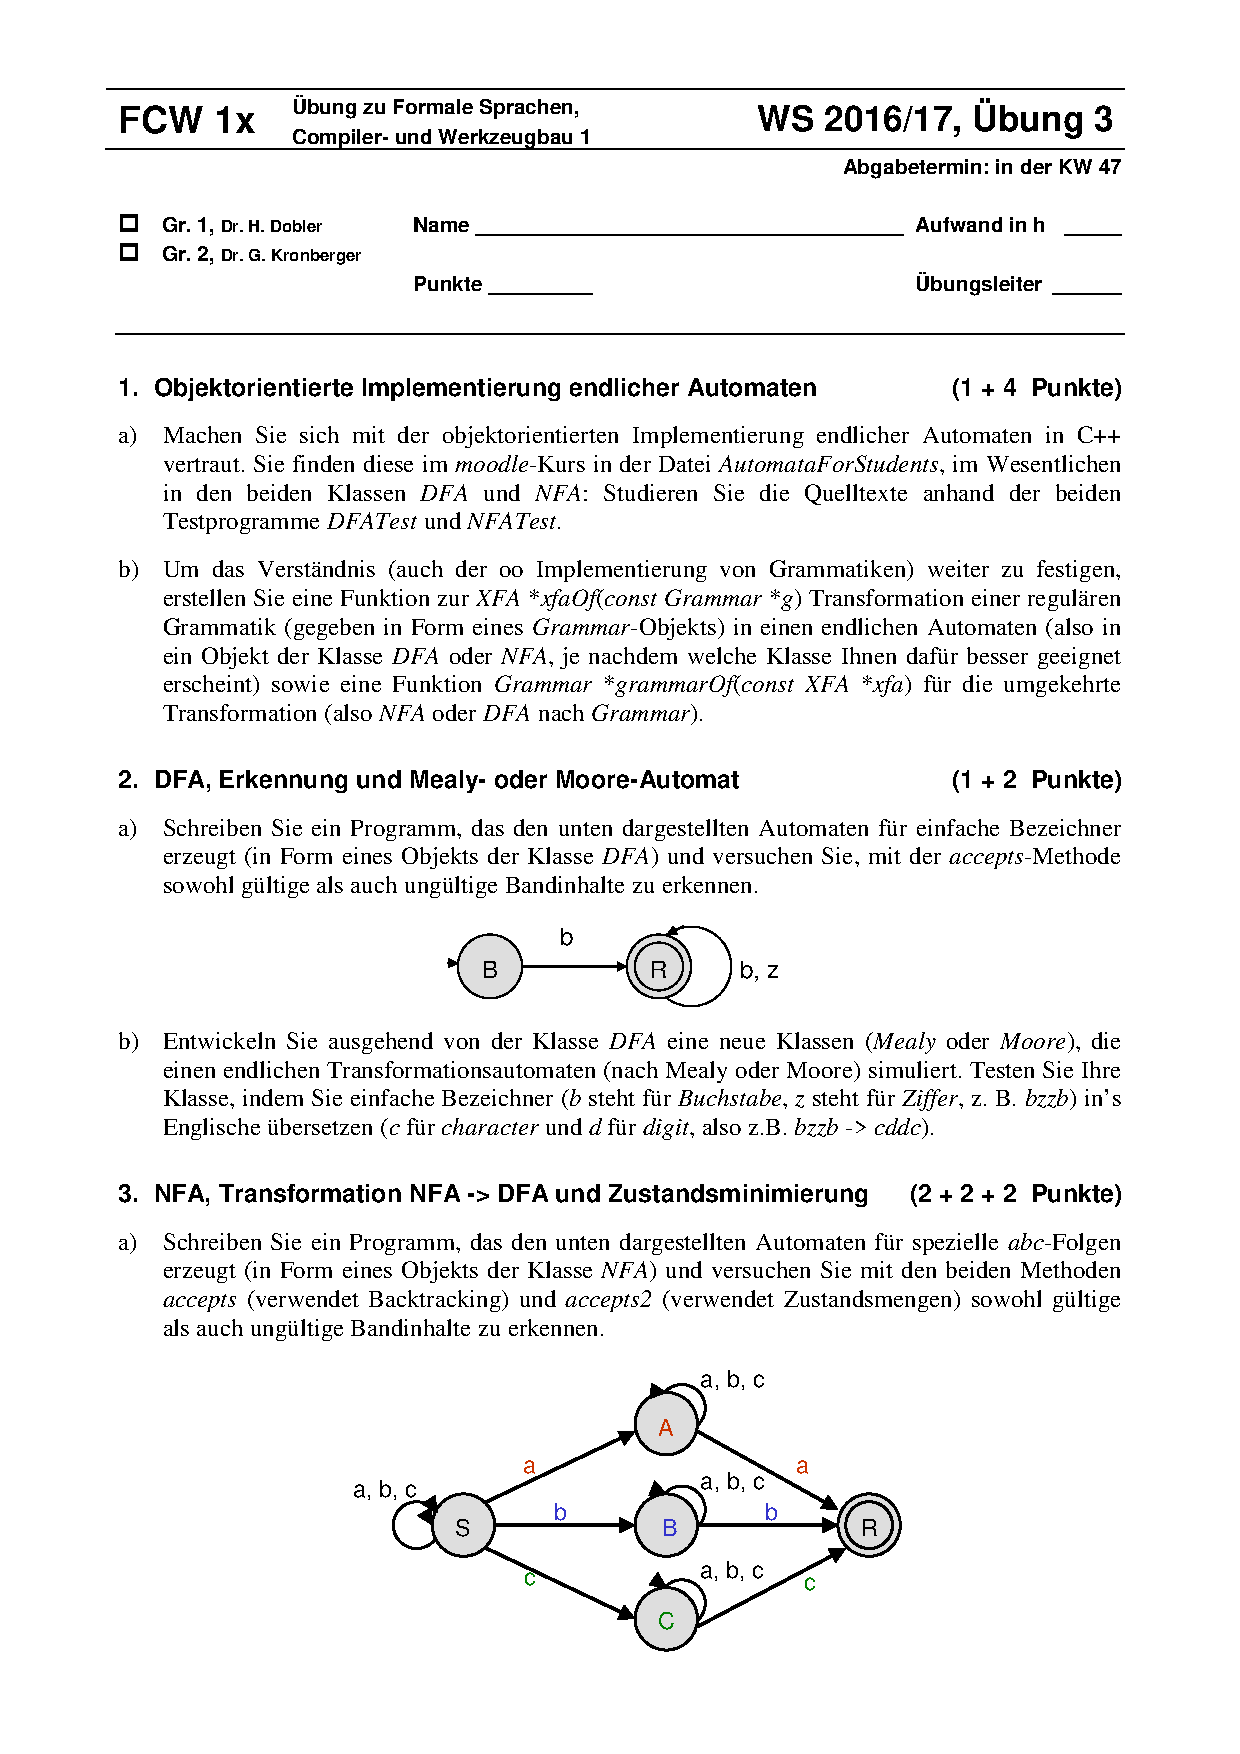
\includepdf[pages={1,3}]{Fcw1x03A.pdf}

% Section gramar and basics 
\section{OO-Implementierung endlicher Automaten}
\label{sec:oo-finite-automat}
Dieser Abschnitt behandelt die Aufgabe 1 der dritten Übung.
\begin{code}
	\caption{AutomateUtil.hpp}
	\cppSourceFile{\srcDir/AutomateUtil.hpp}
\end{code}
\begin{code}
	\caption{AutomateUtil.cpp}
	\cppSourceFile{\srcDir/AutomateUtil.cpp}
\end{code}

\section{DFA und Mealy Automat}
\label{sec:oo-dfa-mealy}
Dieser Abschnitt behandelt die Aufgabe 2 der dritten Übung. Die Konvertierung erfolgt über eine Funktion, die über einen Lambda-Ausdruck der Klasse übergeben werden kann. Die Methode \emph{observeCurrentTapeSymbol} ist eine virtuelle Methode, die der Klasse \emph{DFA} hinzugefügt wurde. In der Methode \emph{accepts} wird beim Setzen des aktuellen Symbols die Beobachtermethode aufgerufen.
\begin{code}
	\caption{Mealy.hpp}
	\cppSourceFile{\srcDir/Mealy.hpp}
\end{code}
\begin{code}
	\caption{TestMealy.cpp}
	\cppSourceFile{\srcDir/TestMealy.cpp}
\end{code}

\begin{figure}[h]
\centering
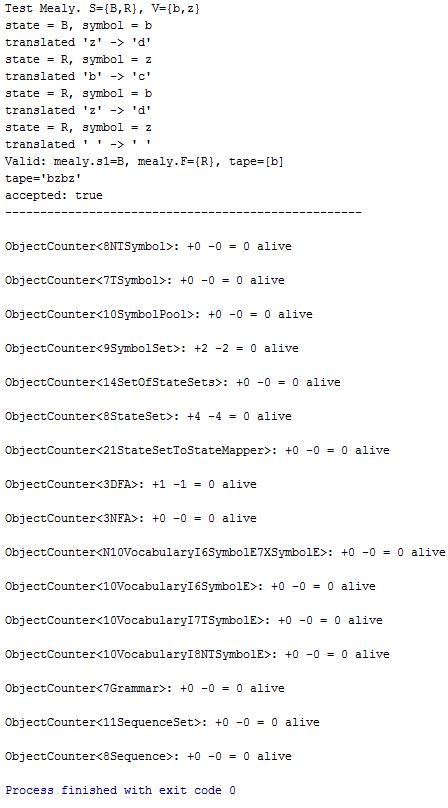
\includegraphics[scale=0.8]{\imageDir/test_mealy.JPG}
\caption{Tests für Mealy Automat}
\label{fig:test-mealy}
\end{figure}
\ \newpage

\section{NFA $\rightarrow$ DFA Transformation und Zustandsminimierung}
\label{sec:oo-nfa-dfa}
Dieser Abschnitt behandelt die Aufgabe 3 der dritten Übung. 

\begin{code}
	\caption{TestNfaToDfa.cpp}
	\cppSourceFile{\srcDir/TestNfaToDfa.cpp}
\end{code}
\ \newpage

\begin{figure}[h]
\centering
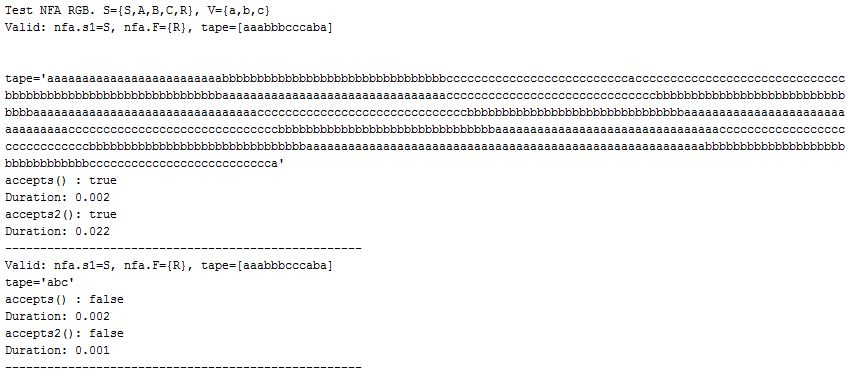
\includegraphics[scale=0.8, angle=90]{\imageDir/test_nfa_dfa.JPG}
\caption{Tests für die beiden Accepts-Methoden}
\label{fig:test-nfa-dfa}
\end{figure}
\ \newline
Es fällt auf, dass die Methode \emph{accepts2} bei langen Bändern deutlich langsamer ist als die Methode \emph{accepts}.
\newpage

\begin{figure}[h]
\centering
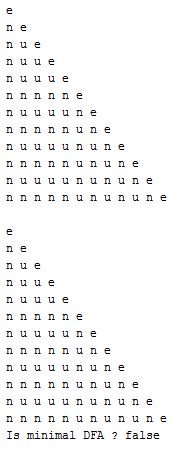
\includegraphics[scale=0.8, angle=90]{\imageDir/test_nfa_dfa_minimal.JPG}
\caption{Tests für minimalen Automaten}
\label{fig:test-nfa-dfa-minimal}
\end{figure}

\begin{figure}[h]
\centering
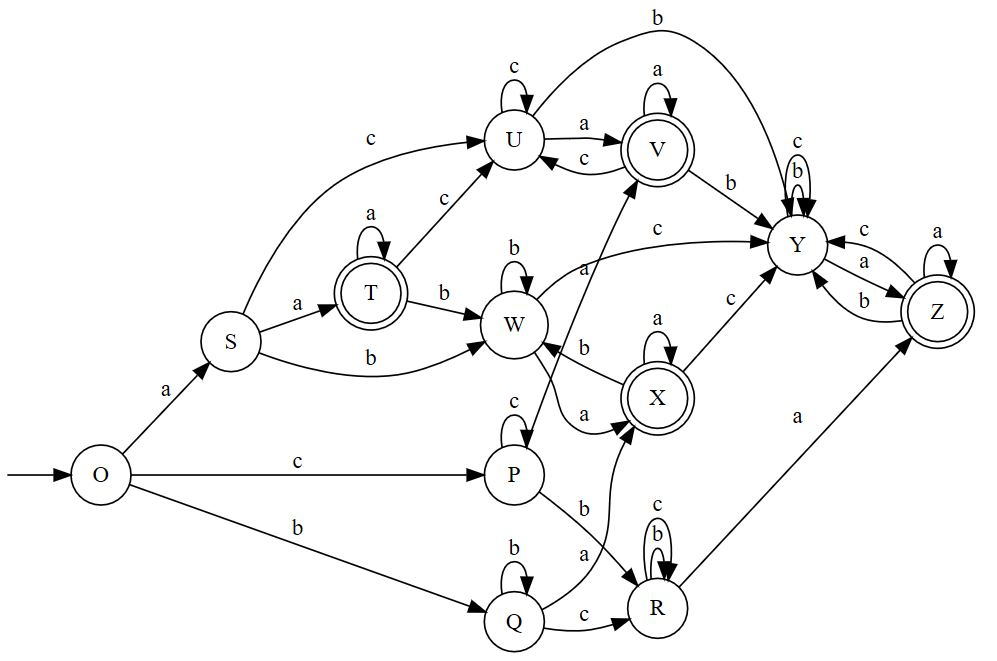
\includegraphics[scale=0.6]{\imageDir/graph-nfa-dfa.JPG}
\caption{Nicht minimaler DFA generiert aus NFA}
\label{fig:graph-nfa-dfa}
\end{figure}
\ \newpage

\begin{figure}[h]
\centering
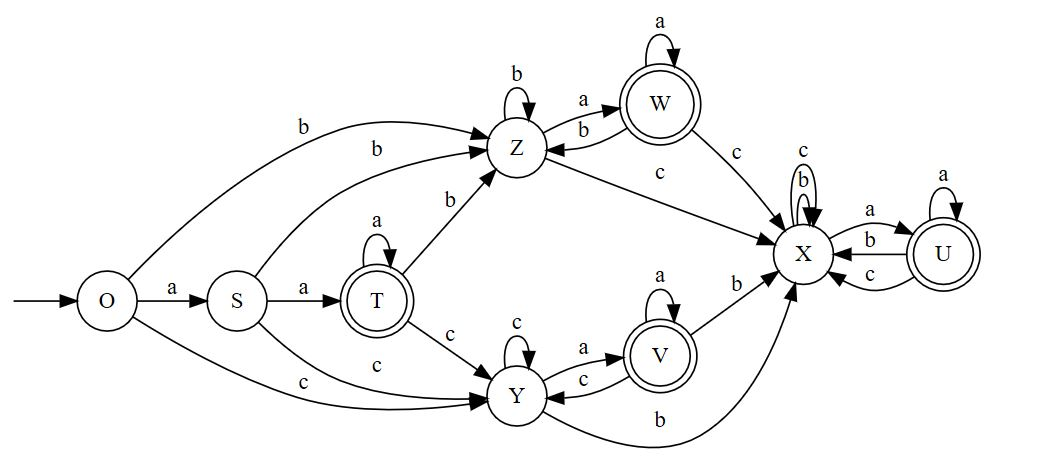
\includegraphics[scale=0.6]{\imageDir/graph-nfa-dfa-minimal.JPG}
\caption{Minimaler DFA generiert aus NFA}
\label{fig:graph-nfa-dfa}
\end{figure}

\section{Kellerautomat und erweiterter Kellerautomat}
\label{sec:oo-stack-automat}
Dieser Abschnitt behandelt die Aufgabe 3 der dritten Übung.
\newline
\newline
Folgende Grammatik ist die gegebene Grammatik in der Schreibweise der formalen Sprachen.
\newline
\newline
\begin{tabularx}{\textwidth}{p{100pt} @{$\rightarrow$ \hspace{20pt}} X}
  Declaration     & VAR $\mid$ VarDeclList \\ 
  VarDeclList     & $\epsilon$ $\mid$ VarDecl ';' VarDeclList \\ 
  VarDecl         & IdentList ':' Type \\ 
  IdentList       & ident $\mid$ RepeatIdentList \\ 
  RepeatIdentList &  $\epsilon$ $\mid$ ',' ident MoreIdentList \\ 
  Type            & OptArray TypeIdent \\ 
  OptArray        & $\epsilon \mid$ ARRAY '(' number ')' OF \\ 
  TypeIdent       &  INTEGER $\mid$ BOOLEAN $\mid$ CHAR 
 \end{tabularx}
\ \newpage
Folgende Tabelle zeigt die Zustandsüberführungsfunktionen des Kellerautomaten.
\newline
\newline
\begin{tabularx}{\textwidth}{X X X X X X}
  \emph{$Zustand_P$} & \emph{$Eingabe_P$} & \emph{$Keller_P$} & \emph{$Zustand_F$} & \emph{$Keller_F$} & \emph{Schritt} \\
  Declaration & VAR         & -    & E1          & -     & 1 \\
  Declaration & $\epsilon$  & -    & VarDeclList & -     & 2 \\
  VarDeclList & $\epsilon$  & -    & E2          & -     & 3 \\
  VarDeclList & $\epsilon$  & \$2  & VarDecl     & \$2   & 4 \\
  \$2         & ;           & -    & VarDeclList & -   & 5 \\
  VarDeclList & $\epsilon$  & -    & E2          & -     & 9 \\
  VarDecl     & $\epsilon$  & \$3  & IdentList   & \$3   & 10 \\
  \$3         & ;           & -    & Type        & -     & 11 \\
  Type        & $\epsilon$  & \$4  & OptArray    & \$4   & 13 \\
  \$4         & $\epsilon$  & -    & TypeIdent   & -     & 14 \\
  TypeIdent   & INTEGER     & -    & E3          & -     & 16 \\
  TypeIdent   & BOOLEAN     & -    & E3          & -     & 17 \\
  TypeIdent   & CHAR        & -    & E3          & -     & 18 \\
  OptArray    & $\epsilon$  & -    & E4          & -     & 20 \\
  OptArray    & ARRAY       & \$5  & -           & \$5   & 21 \\
  \$5         & (           & \$6  & -           & \$6   & 22 \\
  \$6         & number      & \$7  & -           & \$7   & 22 \\
  \$7         & )           & \$8  & -           & \$8   & 22 \\
  \$8         & OF          & -    & E5          & -     & 22 \\
 \end{tabularx}
 
\section{LL(k)-Bedingung und Transformation}
Dieser Abschnitt behandelt die Aufgabe 4 der dritten Übung.
\subsection{Terminale Anfänge und Nachfolger Länge 1}
Folgende Tabelle zeigt die Ermittlung der terminalen Anfänge:
\newline
\newline
\begin{tabularx}{\textwidth}{p{45pt} @{$\rightarrow$ \hspace{1pt}} X p{77pt} @{$=$ \hspace{1mm}} p{60pt}}
progmod  & \textbf{MODULE} id : priority ; imppart block id & First(progmod) & $\{MODULE\}$ \\
priority & \textbf{const} $|$ \textbf{$\epsilon$}           & First(priority)& $\{const, \epsilon\}$ \\
imppart  & \textbf{FROM} id IMPORT implist $|$ \textbf{IMPORT} implist & First(imppart) & $\{FROM, IMPORT\}$\\
implist  & \textbf{id} $|$ \textbf{id} , implist            & First(implist) & $\{id\}$ \\
block    & \textbf{dclpart} statpart $|$ statpart           & First(block)   & $\{dclpart\}$ \\
dclpart  & \textbf{DECL} $|$ \textbf{DECL} ; dclpart        & & $\{DECL\}$ \\
block    & dclpart statpart $|$ \textbf{statpart}           & & $\{statpart\}$ \\
statpart & \textbf{BEGIN} statseq ; END                     & & $\{BEGIN\}$ \\
         &                                                  & & $\{BEGIN, DECL\}$ \\
dclpart  & \textbf{DECL} $|$ \textbf{DECL} ; dclpart        & First(dclpart) & $\{DECL\}$ \\
statpart & \textbf{BEGIN} statseq ; END                     & First(statseq)& $\{BEGIN\}$ \\
statseq  & \textbf{STAT} $|$ \textbf{STAT} ; statseq        & & $\{STAT\}$ \\
\end{tabularx}
\ \newpage
Folgende Tabelle zeigt die Ermittlung der terminalen Nachfolger:
\newline
\newline
\begin{tabularx}{\textwidth}{p{90pt}  @{$=$ \hspace{2mm}} X p{50pt}}
Follow(progmod)  & $\{\}$ \\
Follow(priority) & $\{;\}$ \\
Follow(imppart)  & $\{\} \cup First(block)$ \\
                 & $\{DECL, BEGIN\}$ \\
Follow(implist)  & $\{\} \cup Follow(imppart)$ \\
                 & $\{DECL, BEGIN\}$ \\
Follow(block)    & $\{id\}$ \\
Follow(dclpart)  & $\{\} \cup First(statpart)$ \\
                 & $\{BEGIN\}$ \\
Follow(statpart) & $\{\} \cup Follow(block)$ \\
                 & $\{id\}$ \\
Follow(statseq)  & $\{;\}$ \\
 \end{tabularx}

\subsection{Ist eine LL(k) Grammatik}
Es handelt sich hierbei um eine LL(k)-Grammatik wobei $k>0$, da es Regeln gibt die Optionen haben. Es handelt sich um eine LL(3)-Grammatik da es maximal 3 \emph{Lookahead} benötigt, damit auf ein Terminalsymbol abgeleitet werden kann.

\subsection{Transformation zu einer LL(1)-Grammatik}
\begin{tabularx}{\textwidth}{p{80pt} @{$\rightarrow$ \hspace{20pt}} X}
  progmod         & MODULE id : priority ; imppart block id .\\ 
  priority        & const $|$ $\epsilon$ \\
  imppart         & FROM id IMPORT implist $|$ IMPORT implist \\
  implist         & id implistRest \\
  implistRest     & , id implrest $|$ $\epsilon$ \\
  block           & dclpart statpart $|$ statprt \\
  dclpart         & DECL $|$ DECL ; dclpart \\
  statpart        & BEGIN statseq ; END \\
  statseq         & STAT statseqList \\
  statseqList     & ; statseqList $|$ $\epsilon$
  
 \end{tabularx}
 
\end{document}